\documentclass[UTF8,a4paper]{ctexart}

\usepackage{geometry}
\geometry{left=2.50cm,right=2.50cm,top=2.50cm,bottom=2.50cm}
\usepackage{amsmath,amssymb,bm}
\usepackage{booktabs,longtable,multirow,array,tabularx}
\usepackage{graphicx,float,caption,subcaption,placeins}
\usepackage{fancyhdr}
\usepackage{xcolor}
\usepackage{hyperref}
\usepackage{tikz}
\usetikzlibrary{arrows.meta,positioning,shapes.geometric,calc}
\usepackage{listings}
\usepackage{mdframed}
\usepackage{titlesec}
\usepackage{tocloft}

\setmainfont{Times New Roman}
\renewcommand{\arraystretch}{1.18}
\setlength{\tabcolsep}{5pt}
\captionsetup{font=small,justification=centering,labelsep=quad}
\hypersetup{colorlinks=true,linkcolor=black,citecolor=black,urlcolor=black}
\pagestyle{fancy}
\fancyhf{}
\fancyfoot[C]{\thepage}
\renewcommand{\headrulewidth}{0pt}

\ctexset{
  section={name={,、},number=\chinese{section},format=\centering\heiti\zihao{4}},
  subsection={format=\raggedright\heiti\zihao{-4}},
  subsubsection={format=\raggedright\heiti\zihao{-4}}
}
\titleformat{\paragraph}{\bfseries}{}{0em}{}
\titlespacing{\paragraph}{0pt}{1.5ex}{1ex}
\renewcommand{\cftsecleader}{\cftdotfill{\cftdotsep}}
\renewcommand{\contentsname}{}

\lstset{
  language=C++,basicstyle=\ttfamily\footnotesize,numbers=left,
  numberstyle=\tiny,numbersep=7pt,breaklines=true,showstringspaces=false,
  frame=single,columns=fullflexible,keepspaces=true,
  keywordstyle=\color{blue!70!black},commentstyle=\color{green!45!black}
}

\newcommand{\E}{\mathcal{E}}
\newcommand{\V}{\mathcal{V}}
\newcommand{\eps}{\varepsilon}
\newcommand{\alg}{\textsc{Apex-MOA*}}

\title{\heiti\zihao{3} 城市道路网络多目标通行路径规划与扰动重规划}
\author{}
\date{}

\begin{document}
\zihao{-4}\songti\linespread{1.15}\selectfont
\setcounter{page}{1}

\maketitle
\vspace{-1.8cm}

{\centering\heiti\zihao{3} 摘\quad 要\par}
\vspace{0.6em}

城市道路通行同时受距离、时间、地形起伏、道路结构复杂度与路段数量影响，单目标最优路线通常不能兼顾全部需求。本文将 NY、BAY、COL 三个大规模真实道路网表示为带五维非负边权的有向图，构建“单目标求解---精确 Pareto 搜索---高维近似覆盖---偏好推荐与扰动重规划”的递进式模型。

针对问题一，采用带前驱恢复的 Dijkstra 算法分别求解五类单目标最短路，并以交叉相对代价和路径重合度度量目标冲突。三个城市的 300 组查询中，没有一组的五类最优路径完全相同；BAY 在时间和地形目标上的平均交叉相对代价分别达到 1.876 和 1.849，目标冲突最为突出。

针对问题二，建立三目标字典序多目标 A* 模型。对终点执行三次反向 Dijkstra 构造一致下界，以二维有序 skyline 完成同节点和终点的支配查询；仅在 OPEN 耗尽时确认完整性。90 组查询共得到 3,023,770 个互不相同的精确 Pareto 目标向量，其中 NY、BAY、COL 分别为 1,640,101、556,813、826,856 个。

针对问题三，在统一标签搜索框架中分别处理二、三、五目标问题。二维采用精确搜索；三维和五维采用带真实代表路径的 OPEN 标签合并与终点覆盖剪枝，给出乘性 $\eps=0.20$ 覆盖证书。最终 270 组“查询--维数”组合全部获得保证，共输出 20,669 条完整合法路径。相较基线方法，五维搜索时间中位数由 12.263 秒降至 0.053 秒，标签数中位数由 3,007,743 降至 66,874.5。

针对问题四，以候选集极差归一化构造时间优先、平稳优先、均衡和时间最短四种偏好，并用整系数标量化消除浮点排序误差。封路后，以原图精确距离为一致下界，在剩余完整路网上运行 A* 重规划。指定关闭边下，90 组查询封路前后均可达；360 条原推荐中 292 条受阻，9 组查询的旧候选全部失效但仍可通过全图重规划恢复。最快路线的封路内在损失中位数在 NY、BAY、COL 分别为 4.432\%、8.840\%、5.830\%。全部结果均通过逐边成本复算、内部非支配检查和独立最短路复核。

\vspace{1em}
{\heiti 关键词：}多目标最短路；Pareto 前沿；多目标 A*；乘性近似；偏好推荐；动态重规划

\newpage
{\centering\heiti\zihao{3} 目\quad 录\par}
\vspace{1em}
\tableofcontents

\section{问题背景与重述}

\subsection{研究背景}

实际道路运输决策很少由单一指标决定。距离较短的路线可能因道路等级或路口结构而耗时较长；时间最短路线又可能经过高程变化明显、节点连接复杂的区域。尤其在应急运输、特殊车辆通行和道路临时管制情形下，规划者不仅需要一条最短路，还需要一组能够呈现目标权衡的候选路线，以及在路网发生变化后快速恢复可行方案的能力。

本题给出 NY、BAY、COL 三个城市的真实有向道路网络，每条边包含距离 $c_1$、时间 $c_2$、地形起伏 $c_3$、道路复杂度 $c_4$ 和路段计数 $c_5$ 五项非负成本。三个网络规模达到 26 万至 44 万个节点、73 万至 104 万条有向边，属于大规模最短路基准问题的典型规模\cite{dimacs}。完整枚举路径不可行；而多目标 Pareto 前沿又可能随目标维数快速膨胀。因此，模型必须同时兼顾解的正确性、近似保证、内存开销与扰动响应速度。

\subsection{问题重述}

本文依次解决以下四项任务：

\begin{enumerate}
  \item 对每个给定起终点，分别最小化五项成本，输出完整路径，并比较不同单目标最优路径的冲突程度；
  \item 同时最小化 $(c_1,c_2,c_3)$，求出每组查询全部不同的精确 Pareto 目标向量；
  \item 对前 $m=2,3,5$ 项目标分别构造非支配候选集，在高维情形下使用可证明质量的近似方法，并评价规模、质量、时间和内存；
  \item 从候选集中按不同通行偏好推荐路线；删除指定的 50 条有向边后，在完整剩余路网上重规划，比较可达性、成本变化、推荐质量和计算效率。
\end{enumerate}

\subsection{总体技术路线}

本文四个模型共享同一五维邻接表与路径核验模块。问题一提供五个单目标基准；问题二研究完整三维前沿；问题三通过可认证近似控制高维标签爆炸；问题四把多目标候选转化为可解释的偏好决策，并在封路后进行精确标量重规划。技术路线如图~\ref{fig:route} 所示。

\begin{figure}[H]
\centering
\begin{tikzpicture}[
  node distance=0.65cm and 0.55cm,
  box/.style={draw,rounded corners,minimum width=2.7cm,minimum height=0.9cm,align=center},
  arrow/.style={-{Stealth[length=2mm]},thick}
]
\node[box] (data) {五维有向路网\\查询与封路表};
\node[box,right=of data] (one) {五次 Dijkstra\\单目标基准};
\node[box,right=of one] (two) {精确多目标 A*\\三维 Pareto 前沿};
\node[box,below=of two] (three) {标签合并与覆盖剪枝\\2/3/5维候选集};
\node[box,left=of three] (four) {偏好标量化\\封路后 A* 重规划};
\node[box,left=of four] (verify) {逐边复算\\独立最优性复核};
\draw[arrow] (data)--(one);
\draw[arrow] (one)--(two);
\draw[arrow] (two)--(three);
\draw[arrow] (three)--(four);
\draw[arrow] (four)--(verify);
\draw[arrow,dashed] (data) |- (three);
\draw[arrow,dashed] (data) |- (four);
\end{tikzpicture}
\caption{总体建模与求解流程}
\label{fig:route}
\end{figure}

\section{模型假设、符号与数据处理}

\subsection{基本假设}

\begin{enumerate}
  \item 题目提供的五维边权与有向连接关系准确；封路时仅删除指定方向的边，未列出的反向边仍可通行。
  \item 路径成本具有可加性，且封路后保留边的原始成本不变；道路复杂度不因删边重新计算。
  \item 五项边权均非负，因此含正成本环的路径不可能优于删环后的路径；全零环也只产生重复目标向量，故最优解可取为无重复节点的简单路径。
  \item 问题四给出的偏好权重代表可解释的决策情景，而非对真实用户偏好的统计估计；不同查询采用相同权重含义，但使用各自候选集确定归一化尺度。
\end{enumerate}

\subsection{符号说明}

\begin{table}[H]
\centering
\caption{主要符号}
\begin{tabularx}{0.94\textwidth}{cX}
\toprule
符号 & 含义 \\
\midrule
$G=(\V,\E)$ & 有向道路网络，$\V$ 为节点集，$\E$ 为有向边集 \\
$\bm c(e)$ & 边 $e$ 的五维非负成本向量 $(c_1,\ldots,c_5)$ \\
$P=(v_0,\ldots,v_k)$ & 从 $s=v_0$ 到 $t=v_k$ 的无重复节点路径 \\
$\bm C(P)$ & 路径五维累计成本，$C_j(P)=\sum_{e\in P}c_j(e)$ \\
$g(\ell)$ & 搜索标签 $\ell$ 从起点至当前节点的累计成本 \\
$h(v)$ & 当前节点 $v$ 至终点的逐目标一致下界 \\
$f(\ell)$ & 标签完整路径成本下界，$f=g+h$ \\
$\mathcal P^*$ & 精确 Pareto 前沿 \\
$\eps$ & 乘性近似参数；本文三、五维取 $\eps=0.20$ \\
$L_j,R_j$ & 问题四第 $j$ 项成本的基准值与极差尺度 \\
$W(P)$ & 整系数标量化后的路径评分 \\
\bottomrule
\end{tabularx}
\end{table}

\subsection{数据规模与预处理}

三个城市路网规模如表~\ref{tab:data}。合并边表按起点稳定排序后构造压缩邻接表，同时构造反向图。保留实际边编号，以正确处理同一端点对之间的平行边。任务一使用每城 100 组查询，任务二至四分别使用题目指定的每城 30 组查询，不跨任务替换点对。

\begin{table}[H]
\centering
\caption{数据集规模与查询数}
\label{tab:data}
\begin{tabular}{lrrrr}
\toprule
城市 & 节点数 & 有向边数 & 问题一查询 & 问题二至四查询 \\
\midrule
NY  & 264,346 & 730,100   & 100 & 30 \\
BAY & 321,270 & 794,830   & 100 & 30 \\
COL & 435,666 & 1,042,400 & 100 & 30 \\
\bottomrule
\end{tabular}
\end{table}

每条输出路径均执行四层核验：首尾节点与查询一致；节点不重复；相邻节点对应真实有向边；五项成本由实际边逐项重算并与输出一致。对 Pareto 集进一步检查目标向量唯一性和内部非支配性。

\section{问题一：单目标路径与目标冲突}

\subsection{单目标最短路模型}

对目标 $i\in\{1,\ldots,5\}$，建立模型
\begin{align}
\min_{P}\quad & C_i(P)=\sum_{e\in P}c_i(e),\\
\text{s.t.}\quad & v_0=s,\quad v_k=t,\\
& (v_{r-1},v_r)\in\E,\quad r=1,\ldots,k,\\
& v_p\neq v_q,\quad 0\le p<q\le k.
\end{align}
由于边权非负，Dijkstra 算法\cite{dijkstra} 适用。每个查询对五项目标分别运行一次二叉堆 Dijkstra；目标节点首次出队时提前终止，并用前驱节点及实际边编号恢复路径。单次最坏时间复杂度为 $O((|\V|+|\E|)\log|\V|)$，工作空间为 $O(|\V|+|\E|)$。

\subsection{冲突评价指标}

对查询 $q$，记以第 $i$ 项为目标所得路径为 $P_i^{(q)}$。其在第 $j$ 项上的交叉相对代价定义为
\begin{equation}
R_{ij}^{(q)}=\frac{C_j(P_i^{(q)})}{C_j(P_j^{(q)})}\ge 1.
\end{equation}
$R_{ij}$ 越大，表示优化目标 $i$ 对目标 $j$ 付出的机会成本越高。另以路径边集 Jaccard 系数
\begin{equation}
J_{ik}^{(q)}=\frac{|E(P_i^{(q)})\cap E(P_k^{(q)})|}
{|E(P_i^{(q)})\cup E(P_k^{(q)})|}
\end{equation}
衡量路线结构相似性，并统计同一查询产生的不同完整路径数量。

\subsection{结果分析}

三个城市共输出 $3\times100\times5=1500$ 条合法路径。所有 300 组查询中，五种目标得到的路径均未完全相同，且每组不同路径数的中位数均为 5，说明单一指标之间存在普遍而非偶发的冲突。

表~\ref{tab:q1regret} 给出把五类单目标路径放到各评价维度上计算后的平均与 95\% 分位交叉相对代价。对角线比值恒为 1，表中每列汇总全部五类路线。BAY 的时间和起伏平均相对代价最高，且起伏的 95\% 分位达到 4.134；说明在该路网中，若只优化其他指标，极端情况下会显著牺牲地形平稳性。NY 总体冲突相对较弱，COL 介于两者之间。

\begin{table}[H]
\centering
\caption{问题一交叉相对代价统计}
\label{tab:q1regret}
\resizebox{0.98\textwidth}{!}{
\begin{tabular}{llccccc}
\toprule
城市 & 统计量 & 距离 & 时间 & 起伏 & 复杂度 & 边数 \\
\midrule
NY  & 平均值 & 1.184 & 1.491 & 1.532 & 1.381 & 1.301 \\
    & 95\%分位 & 1.503 & 2.442 & 2.266 & 2.290 & 1.944 \\
BAY & 平均值 & 1.242 & 1.876 & 1.849 & 1.372 & 1.349 \\
    & 95\%分位 & 1.743 & 3.133 & 4.134 & 2.084 & 2.041 \\
COL & 平均值 & 1.194 & 1.630 & 1.459 & 1.404 & 1.376 \\
    & 95\%分位 & 1.574 & 2.684 & 2.310 & 2.172 & 2.084 \\
\bottomrule
\end{tabular}}
\end{table}

因此，直接选择某一单目标最优路会隐含较强偏好，不能替代多目标候选集。问题二和问题三进一步保留互不支配的权衡方案。

\section{问题二：三目标精确 Pareto 前沿}

\subsection{多目标标签模型}

本文在经典多目标标签设置\cite{martins,namoadr} 上，同时最小化距离、时间和起伏。对向量 $\bm x,\bm y\in\mathbb{R}^3$，定义 $\bm x\preceq\bm y$ 当且仅当 $x_j\le y_j$ 对所有 $j$ 成立；若进一步有 $\bm x\ne\bm y$，则称 $\bm x$ 支配 $\bm y$\cite{pareto}，完全相等的向量按重复项处理。

标签写为 $\ell=(v,\bm g)$，其中 $v$ 是当前节点，$\bm g\in\mathbb{Z}_{\ge0}^3$ 是从 $s$ 到 $v$ 的累计成本。若同节点标签 $\ell_a$ 满足
\begin{equation}
\bm g_a\preceq\bm g_b,
\end{equation}
则 $\ell_b$ 加上任意相同后缀都不会优于 $\ell_a$，可以安全删除。

对终点 $t$ 的反向图分别以三项边权运行 Dijkstra，得到
\begin{equation}
h_j(v)=\min_{P:v\leadsto t}C_j(P),\qquad j=1,2,3.
\end{equation}
每一维均满足一致性
\begin{equation}
h_j(u)\le c_j(u,v)+h_j(v),
\end{equation}
故标签下界 $\bm f=\bm g+\bm h(v)$ 沿扩展方向逐维不减。OPEN 按内部顺序 $(c_2,c_1,c_3)$ 的 $\bm f$ 字典序弹出，输出仍恢复为原始 $(c_1,c_2,c_3)$ 顺序。

\subsection{二维 skyline 支配结构}

在多目标 A* 的字典序搜索下\cite{namoadr,dimreduce}，OPEN 的第一内部坐标是 $f_2=g_2+h_2(v)$。对同一节点 $v$，$h_2(v)$ 为常数，因此已出队标签的 $g_2$ 不大于当前标签，支配判断可降为余下二维。维护按第二坐标递增、第三坐标严格递减的 skyline：用二分查找前驱即可判断是否存在支配者；插入后删除被新点覆盖的连续区间。支配查询为 $O(\log k)$，数组区间移动最坏为 $O(k)$，其中 $k$ 是该节点当前 skyline 大小。

初始可行路径只作为终点上界。对其与标签下界的比较仍使用完整三维支配，不能把未按弹出顺序产生的种子提前塞入二维终点索引。目标向量相同只保留一个代表。

\subsection{完整性论证}

算法仅执行三类剪枝：同节点精确支配、已知终点解对 $\bm f$ 的精确支配、重复目标向量删除。由于 $\bm h$ 是逐维可行下界，若某终点解支配 $\bm f$，则它也支配该前缀的任意补全路径；故剪枝不会移除新的 Pareto 向量。边权非负使含环路径总能删去一个环而不增加任一目标，因此每个最优向量都存在简单路径代表；零成本环产生的相同标签则被重复项规则删除。OPEN 耗尽时，所有未被安全剪枝的路径前缀均已处理；反之，OPEN 中尚存标签时仍可能补全出新的终点向量。因此仅在 OPEN 耗尽后，终点集合才恰为完整精确 Pareto 前沿。

\subsection{实验结果}

90 组查询全部以 OPEN 耗尽结束，共得到 3,023,770 个精确向量。实验在双路 Xeon Gold 6430、128 逻辑 CPU、约 125 GiB 内存的 Linux 服务器上以 16 个工作进程批处理；下文时间为单查询搜索阶段的墙钟时间，内存为相应工作进程的峰值 RSS。表~\ref{tab:q2} 表明 NY 单组前沿约 5.4 万个，明显大于 BAY 和 COL，是本题三目标精确搜索的主要计算压力来源。全部查询的搜索耗时中位数为 139.218 秒，最大为 222.674 秒；进程峰值内存中位数 164 MiB，最大 202 MiB。

\begin{table}[H]
\centering
\caption{问题二精确 Pareto 前沿规模}
\label{tab:q2}
\begin{tabular}{lrrrrr}
\toprule
城市 & 查询数 & 向量总数 & 单组最小 & 单组中位数 & 单组最大 \\
\midrule
NY  & 30 & 1,640,101 & 53,917 & 53,926 & 57,526 \\
BAY & 30 &   556,813 & 15,701 & 18,805 & 23,021 \\
COL & 30 &   826,856 & 26,625 & 26,816 & 34,947 \\
\midrule
合计 & 90 & 3,023,770 & -- & -- & -- \\
\bottomrule
\end{tabular}
\end{table}

\begin{table}[H]
\centering
\caption{问题二分城市搜索资源统计}
\label{tab:q2resource}
\begin{tabular}{lrrrr}
\toprule
城市 & 耗时中位数/s & 耗时范围/s & 内存中位数/MiB & 最大内存/MiB \\
\midrule
NY  & 197.69 & 126.77--222.67 & 164 & 171 \\
BAY & 141.35 & 100.44--176.28 & 193 & 202 \\
COL &  91.67 &  74.73--121.24 & 138 & 143 \\
\bottomrule
\end{tabular}
\end{table}

为直观比较三维前沿形态，在每个城市中选取“前沿规模最接近该城市中位数”的查询作为代表，分别为 NY/0001、BAY/0003 和 COL/0001。为消除城市尺度差异，将各坐标按该查询对应目标的单目标最小值归一化：
\begin{equation}
\widetilde C_j(P)=\frac{C_j(P)}{\min_{Q}C_j(Q)},\qquad j=1,2,3.
\end{equation}
图~\ref{fig:q2front} 展示全部精确 Pareto 向量而非抽样点：横、纵坐标分别为归一化距离和时间，颜色表示归一化起伏。这种二维投影避免了三维视角遮挡，仍同时保留三项成本信息。三座城市的前沿都呈弯曲、多分支分布，而非一条可由单个权重参数完整刻画的直线；改善距离、时间中的一项通常伴随另一项或起伏成本上升。NY 和 BAY 的归一化起伏范围可超过 3，而 COL 代表查询的起伏主要位于 1--1.3 之间，说明相同三目标在不同路网中的冲突尺度并不一致。

\begin{figure}[H]
\centering
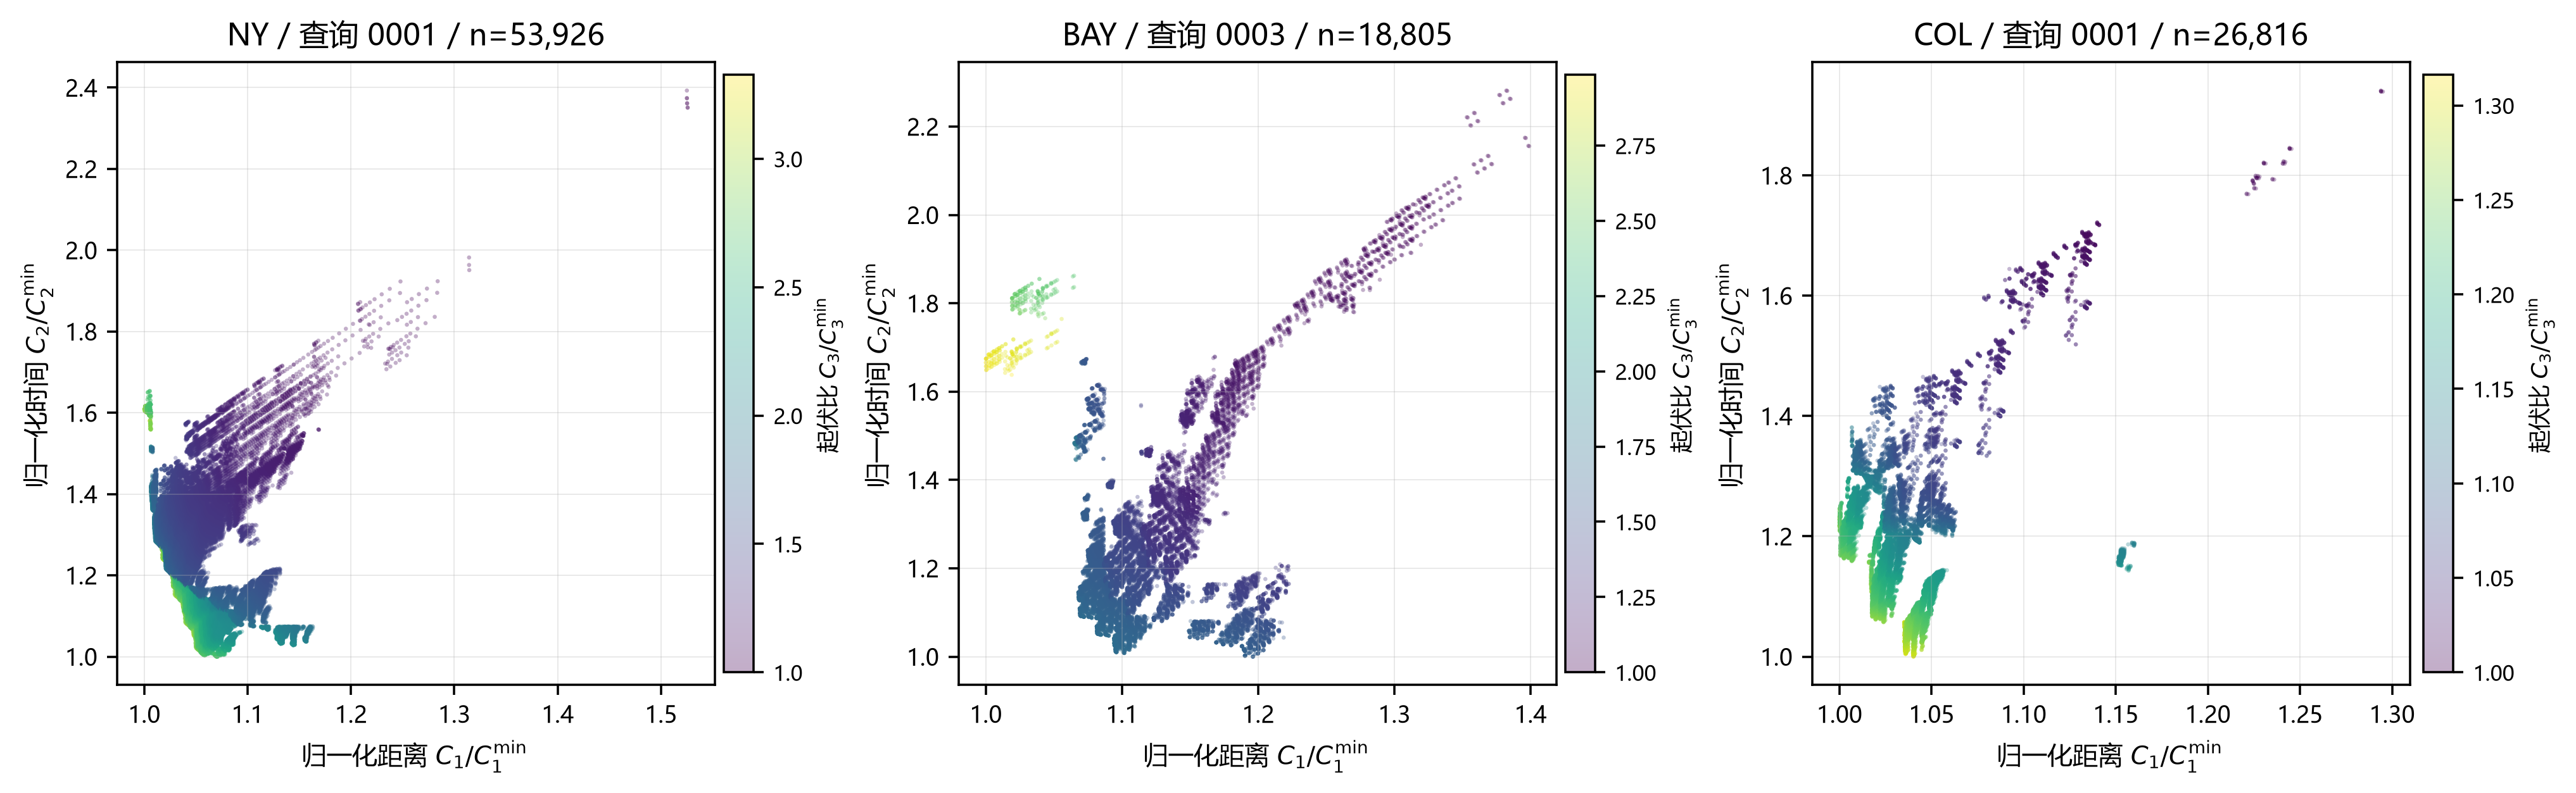
\includegraphics[width=\textwidth]{../figures/q2_pareto_front_examples.png}
\caption{三座城市代表查询的精确 Pareto 前沿（颜色表示归一化起伏）}
\label{fig:q2front}
\end{figure}

图~\ref{fig:q2scale} 左侧进一步给出每城 30 组查询的前沿规模分布，城市间形成清晰层次；右侧将前沿规模与精确搜索时间对应。NY 虽然前沿规模集中在约 5.4 万，但搜索时间仍出现明显差异；COL 的前沿规模普遍高于 BAY，搜索时间却整体更低。因此，输出规模是计算开销的重要因素，但节点标签分布、支配剪枝效率与路网结构同样影响耗时，不能仅用最终向量数预测搜索难度。

\begin{figure}[H]
\centering
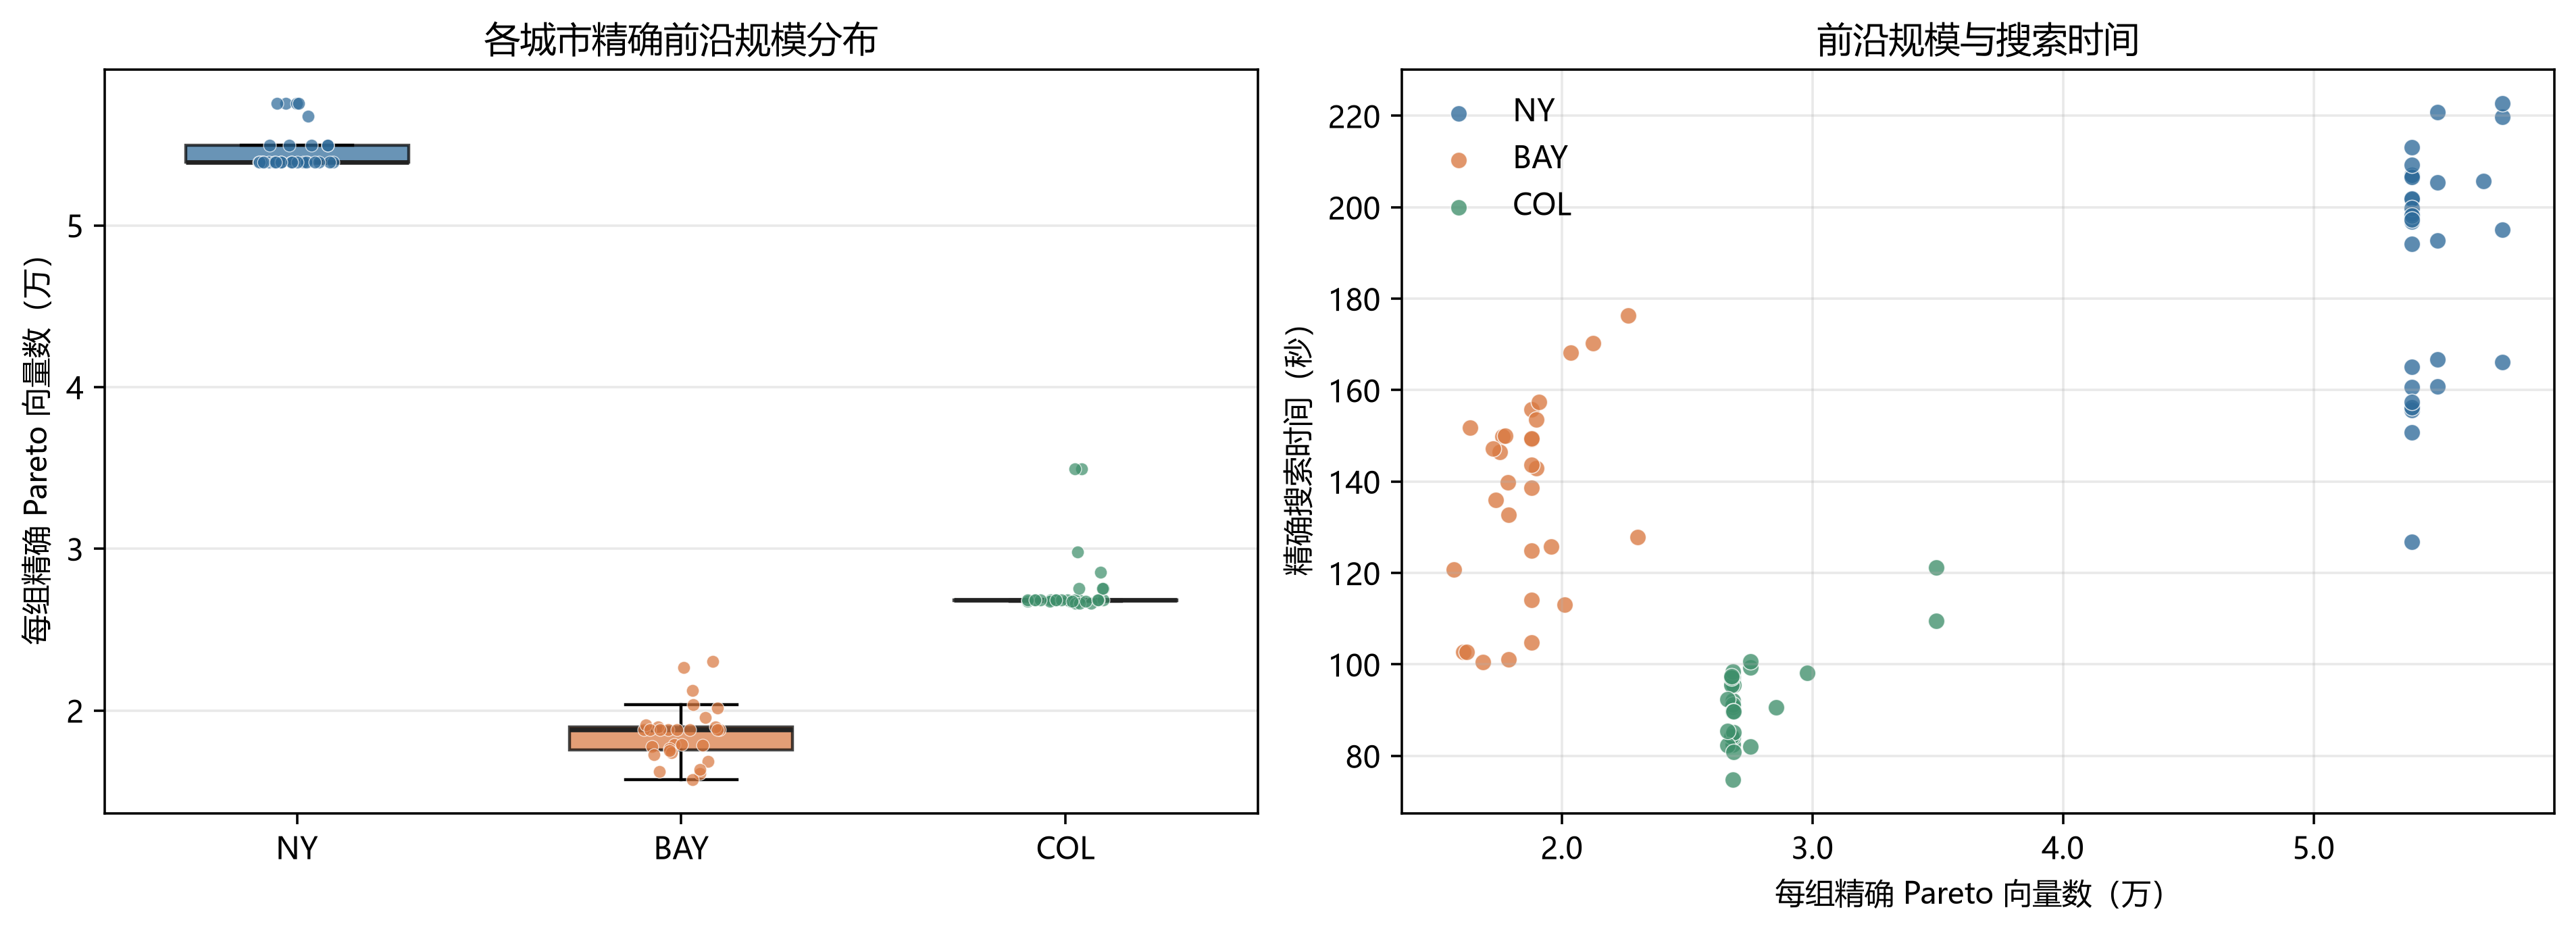
\includegraphics[width=0.98\textwidth]{../figures/q2_front_size_and_time.png}
\caption{三目标精确前沿规模分布及其与搜索时间的关系}
\label{fig:q2scale}
\end{figure}

综合而言，三目标前沿在大规模道路网中已经达到万级，且具有明显的非线性、多分支权衡结构；若继续增加维度并要求完整精确前沿，标签数量与输出规模都可能失控。因此问题三采用“二维精确、三五维有证书近似”的分层策略。

\section{问题三：高维 Pareto 候选与近似求解}

\subsection{统一搜索框架}

对 $m\in\{2,3,5\}$，标签保存当前节点、五维真实累计成本、父标签和实际入边；支配判断只使用前 $m$ 项，但输出完整五项成本。每个参与目标由反向 Dijkstra 给出 $h_j$。由各单目标最短路和归一化随机权重和最短路产生最多 12 条初始可行路径；加权和仅用于提供上界，不作为 Pareto 前沿的替代。

二维模式取 $\eps=0$ 并耗尽 OPEN，得到精确前沿。三维、五维使用 $\eps=0.20$ 的 \alg{} 标签合并\cite{apex}。每个 OPEN 标签额外保存它所代表前缀集合的逐坐标下界 $\bm A$。若两个同节点标签合并，则
\begin{equation}
\bm A_{\rm new}=\min(\bm A_1,\bm A_2),
\end{equation}
并且至少有一条真实代表路径 $\bm g$ 满足
\begin{equation}
g_j+h_j\le(1+\eps)(A_{{\rm new},j}+h_j),
\qquad j=1,\ldots,m.\label{eq:merge}
\end{equation}
是否满足式~\eqref{eq:merge} 使用 128 位整数交叉相乘判断，避免浮点误差。若两条代表都满足，选择最大坐标比值更小者，以保留后续合并余量。

\subsection{终点覆盖剪枝与误差保证}

对标签完整路径下界 $\bm f=\bm g+\bm h$，仅当存在同一条已经恢复的完整路径 $a$，满足
\begin{equation}
C_j(a)\le(1+\eps)f_j,\qquad j=1,\ldots,m,
\end{equation}
时才剪枝。不能把不同路径的各维最小值拼成虚构上界。

式~\eqref{eq:merge} 约束的是累计成本，不是每次扩展都乘一次 $1+\eps$。扩展同一条边时，真实成本和下界同步增加同一非负向量；再次合并时重新对累计下界检验，因此误差不会沿路径累积为 $(1+\eps)^k$。当 OPEN 耗尽时，对真实 Pareto 前沿的任一路径，返回集中都存在一条真实可行路径逐维不超过其 $1.2$ 倍。

\subsection{质量指标}

采用乘性覆盖指标
\begin{equation}
I_\eps(A,R)=\max_{r\in R}\min_{a\in A}
\left[\max\left(1,\max_{j\le m}\frac{C_j(a)}{C_j(r)}\right)-1\right].
\end{equation}
二维以真实精确前沿作为 $R$；三、五维除理论证书外，还以所有已测试配置的非支配并集作经验参考。经验指标只能比较已观察解，不能代替对未知真实前沿的覆盖证书。

\subsection{结果与维数效应}

最终 270 组组合全部得到证书。二维 90 组为精确前沿，三维与五维各 90 组为 $\eps=0.20$ 覆盖集。总计输出 20,669 条路径，其中二维 18,487 条、三维 856 条、五维 1,326 条。表~\ref{tab:q3size} 给出分城市规模。

\begin{table}[H]
\centering
\caption{问题三最终候选路径规模}
\label{tab:q3size}
\begin{tabular}{lrrrrrr}
\toprule
\multirow{2}{*}{城市} & \multicolumn{2}{c}{二维精确} & \multicolumn{2}{c}{三维 $\eps=0.20$} & \multicolumn{2}{c}{五维 $\eps=0.20$}\\
\cmidrule(lr){2-3}\cmidrule(lr){4-5}\cmidrule(lr){6-7}
& 总数 & 单组中位数 & 总数 & 单组中位数 & 总数 & 单组中位数 \\
\midrule
NY  & 2,615  & 41  & 282 & 10 & 482 & 11.5 \\
BAY & 4,051  & 66  & 289 & 10 & 430 & 12 \\
COL & 11,821 & 204 & 285 & 10 & 414 & 12 \\
\midrule
合计 & 18,487 & -- & 856 & -- & 1,326 & -- \\
\bottomrule
\end{tabular}
\end{table}

近似集规模不随维数单调增长，因为三、五维使用 20\% 覆盖压缩，而二维输出完整精确前沿。若比较相同基线算法的资源开销，五维标签爆炸十分明显。表~\ref{tab:q3perf} 显示，OPEN 标签合并把五维搜索时间中位数降低约 99.6\%，标签数中位数降低约 97.8\%；三维也由 83/90 组获证书提升为 90/90 组。默认内部顺序完成 269 组，COL/0017 五维改用起伏优先顺序后完成，未放宽 $\eps$ 或资源上限。

\begin{table}[H]
\centering
\caption{问题三优化前后资源对比（同服务器）}
\label{tab:q3perf}
\begin{tabular}{lrrr}
\toprule
五维指标（90组中位数） & 基线方法 & 标签合并后 & 变化 \\
\midrule
搜索时间/秒 & 12.263 & 0.053 & $-99.6\%$ \\
含加载与初始解总时间/秒 & 14.251 & 1.775 & $-87.5\%$ \\
单进程峰值内存/MiB & 306.5 & 89.0 & $-71.0\%$ \\
累计标签数 & 3,007,743 & 66,874.5 & $-97.8\%$ \\
\bottomrule
\end{tabular}
\end{table}

需注意，基线包含 42 个达到 30 秒上限的五维配置，不能由上述比值推断其最终精确完成时间；优化后五维最大峰值内存仍可能达到约 1055 MiB，也不能声称每个查询的内存均下降。

\section{问题四：方案推荐与封路重规划}

\subsection{候选集合并与固定归一化}

对每个查询合并问题三二维、三维、五维的已认证路径，按五维成本去重并执行五维精确去支配，得到原始候选集 $A$。候选集只负责表达原图中的多目标权衡，封路后的最终路线仍在完整剩余路网中求解。对第 $j$ 项成本定义
\begin{equation}
L_j=\min_{P\in A}C_j(P),\qquad
R_j=\max\left\{1,\max_{P\in A}C_j(P)-L_j\right\}.
\end{equation}
在权重 $\bm w$ 下，推荐评分为
\begin{equation}
S_{\bm w}(P)=\sum_{j=1}^5\bar w_j\frac{C_j(P)-L_j}{R_j},
\qquad \sum_j\bar w_j=1.\label{eq:score}
\end{equation}
四种偏好见表~\ref{tab:weights}。平稳优先强调起伏和复杂度代理指标，并不等同于真实安全风险最小。

\begin{table}[H]
\centering
\caption{推荐偏好权重}
\label{tab:weights}
\begin{tabular}{lccccc}
\toprule
方案 & 距离 & 时间 & 起伏 & 复杂度 & 边数 \\
\midrule
时间优先 & 0.10 & 0.60 & 0.10 & 0.10 & 0.10 \\
平稳优先 & 0.10 & 0.15 & 0.35 & 0.25 & 0.15 \\
均衡     & 0.20 & 0.20 & 0.20 & 0.20 & 0.20 \\
时间最短 & 0    & 1.00 & 0    & 0    & 0 \\
\bottomrule
\end{tabular}
\end{table}

封路前后固定使用同一组 $L_j,R_j$ 与权重，不对封路后的成本重新归一化，也不把超出原候选范围的值截断。式中取 $R_j\ge1$ 可避免某项成本在候选集内无差异时除零。固定尺度使两种路网状态下的评分保持可比，封路后某项超出原范围则如实反映为大于 1 的归一化代价。

\subsection{精确整数标量化}

令表中百分比整数权重为 $w_j=100\bar w_j$，$D$ 为各 $R_j$ 的最小公倍数，定义
\begin{equation}
a_j=\frac{w_jD}{R_j},\qquad
W(P)=\sum_{j=1}^{5}a_jC_j(P).
\end{equation}
由于 $\sum_j w_jL_j/R_j$ 对同一查询是常数，最小化 $W$ 与最小化式~\eqref{eq:score} 完全等价。程序用 128 位整数并显式检查溢出，避免浮点舍入改变路径排序。特别地，$L_j$ 是整条路径评分中的常数，不能在每条边上重复相减。

\subsection{封路后 A* 重规划}

每城市删除封路表中 50 个有向端点对对应的全部边，平行边一并删除。首先从问题三全部原候选中筛出未经过关闭边的路径，作为可行上界；随后在原图上对当前标量边权运行反向 Dijkstra，得到原图至终点的精确距离 $h_0(v)$。删边只会收缩可行域，因此
\begin{equation}
h_0(v)\le h_D(v),
\end{equation}
且 $h_0$ 在所有保留边上仍一致，可作为中断图 A* 的下界\cite{astar}。因此，筛出的存活旧路径提供可行上界，$h_0$ 提供节点下界，A* 则在完整剩余图上缩小两者间的差距，而非只在旧候选中选择。当 OPEN 最小下界不小于已有上界或目标出队时得到精确标量最优解；若无上界且 OPEN 耗尽，才判定不可达。

\subsection{评价指标}

记原候选推荐值为 $W_A$，原图全局最优值为 $W_0^*$，封路后全局最优值为 $W_D^*$。分别计算
\begin{align}
G_{\rm cand}&=W_A/W_0^*-1 &&\text{（原候选相对误差）},\\
L_{\rm close}&=W_D^*/W_0^*-1 &&\text{（封路内在损失）},\\
\Delta_{\rm user}&=W_D^*/W_A-1 &&\text{（用户推荐相对变化）}.
\end{align}
这三个量必须区分：$W_D^*$ 可能低于近似候选值 $W_A$，但一定不低于 $W_0^*$。因此封路后评分下降可能只是重规划消除了候选近似误差，不能解释为删边改善了路网。

\subsection{可达性与总体扰动影响}

三座城市封路前后 90 组查询全部可达。360 条原推荐中有 292 条经过关闭边；9 组查询的全部旧候选失效，但全图 A* 仍找到新路线。若仅在旧候选中筛选，将把这些查询错误判为不可达。

\begin{table}[H]
\centering
\caption{封路后的可达性与原方案受阻情况}
\label{tab:q4reach}
\begin{tabular}{lrrrr}
\toprule
城市 & 原图可达 & 封路后可达 & 全部旧候选失效 & 原推荐受阻/120 \\
\midrule
NY  & 30/30 & 30/30 & 7 & 106 \\
BAY & 30/30 & 30/30 & 1 & 95 \\
COL & 30/30 & 30/30 & 1 & 91 \\
\bottomrule
\end{tabular}
\end{table}

表~\ref{tab:q4loss} 给出封路内在损失中位数。时间最短路线在全部 90 组中均受阻且最短时间严格增加，BAY 的中位损失最大；COL 的最坏单组时间最短损失达到 42.232\%。平稳优先和均衡方案的加权损失中位数较小，但由于评价函数不同，不能据此断言其每一项成本都更鲁棒。

\begin{table}[H]
\centering
\caption{封路内在相对损失中位数}
\label{tab:q4loss}
\begin{tabular}{lrrrr}
\toprule
城市 & 时间优先 & 平稳优先 & 均衡 & 时间最短 \\
\midrule
NY  & 3.518\% & 1.134\% & 1.701\% & 4.432\% \\
BAY & 6.480\% & 0.448\% & 0.730\% & 8.840\% \\
COL & 2.406\% & 0.708\% & 0.352\% & 5.830\% \\
\bottomrule
\end{tabular}
\end{table}

\subsection{偏好收益与成本}

表~\ref{tab:tradeoff} 将原图各推荐与同查询时间最短路线比较。时间优先只增加约 1\%--2\% 的时间，便可使起伏和复杂度降低约 3\%--7\%；平稳优先进一步降低代理指标，但 BAY 的时间代价中位数达到 41.447\%。这说明固定平稳权重并不适用于所有用户：若存在明确的最大可接受时间增幅，应改建带时间约束的多目标决策模型。

\begin{table}[H]
\centering
\caption{原图推荐相对时间最短路线的配对变化中位数}
\label{tab:tradeoff}
\begin{tabular}{llrrr}
\toprule
城市 & 方案 & 时间变化 & 起伏变化 & 复杂度变化 \\
\midrule
NY  & 时间优先 & 2.126\% & $-6.430\%$ & $-4.083\%$ \\
NY  & 平稳优先 & 12.519\% & $-14.460\%$ & $-10.130\%$ \\
BAY & 时间优先 & 1.122\% & $-4.107\%$ & $-2.819\%$ \\
BAY & 平稳优先 & 41.447\% & $-26.074\%$ & $-20.319\%$ \\
COL & 时间优先 & 1.756\% & $-4.487\%$ & $-7.164\%$ \\
COL & 平稳优先 & 28.291\% & $-15.570\%$ & $-20.277\%$ \\
\bottomrule
\end{tabular}
\end{table}

图~\ref{fig:q4overview} 左侧给出 360 个“查询--偏好”实例的封路内在损失分布。时间最短方案不仅中位损失较大，也出现更长的上尾；但不同偏好的评价函数不同，因此箱线高低只能在各自偏好含义下解释。右侧以时间最短路线为基准，清楚显示时间优先仅付出少量时间代价，而平稳优先获得更大起伏与复杂度改善时，可能显著增加通行时间。

\begin{figure}[H]
\centering
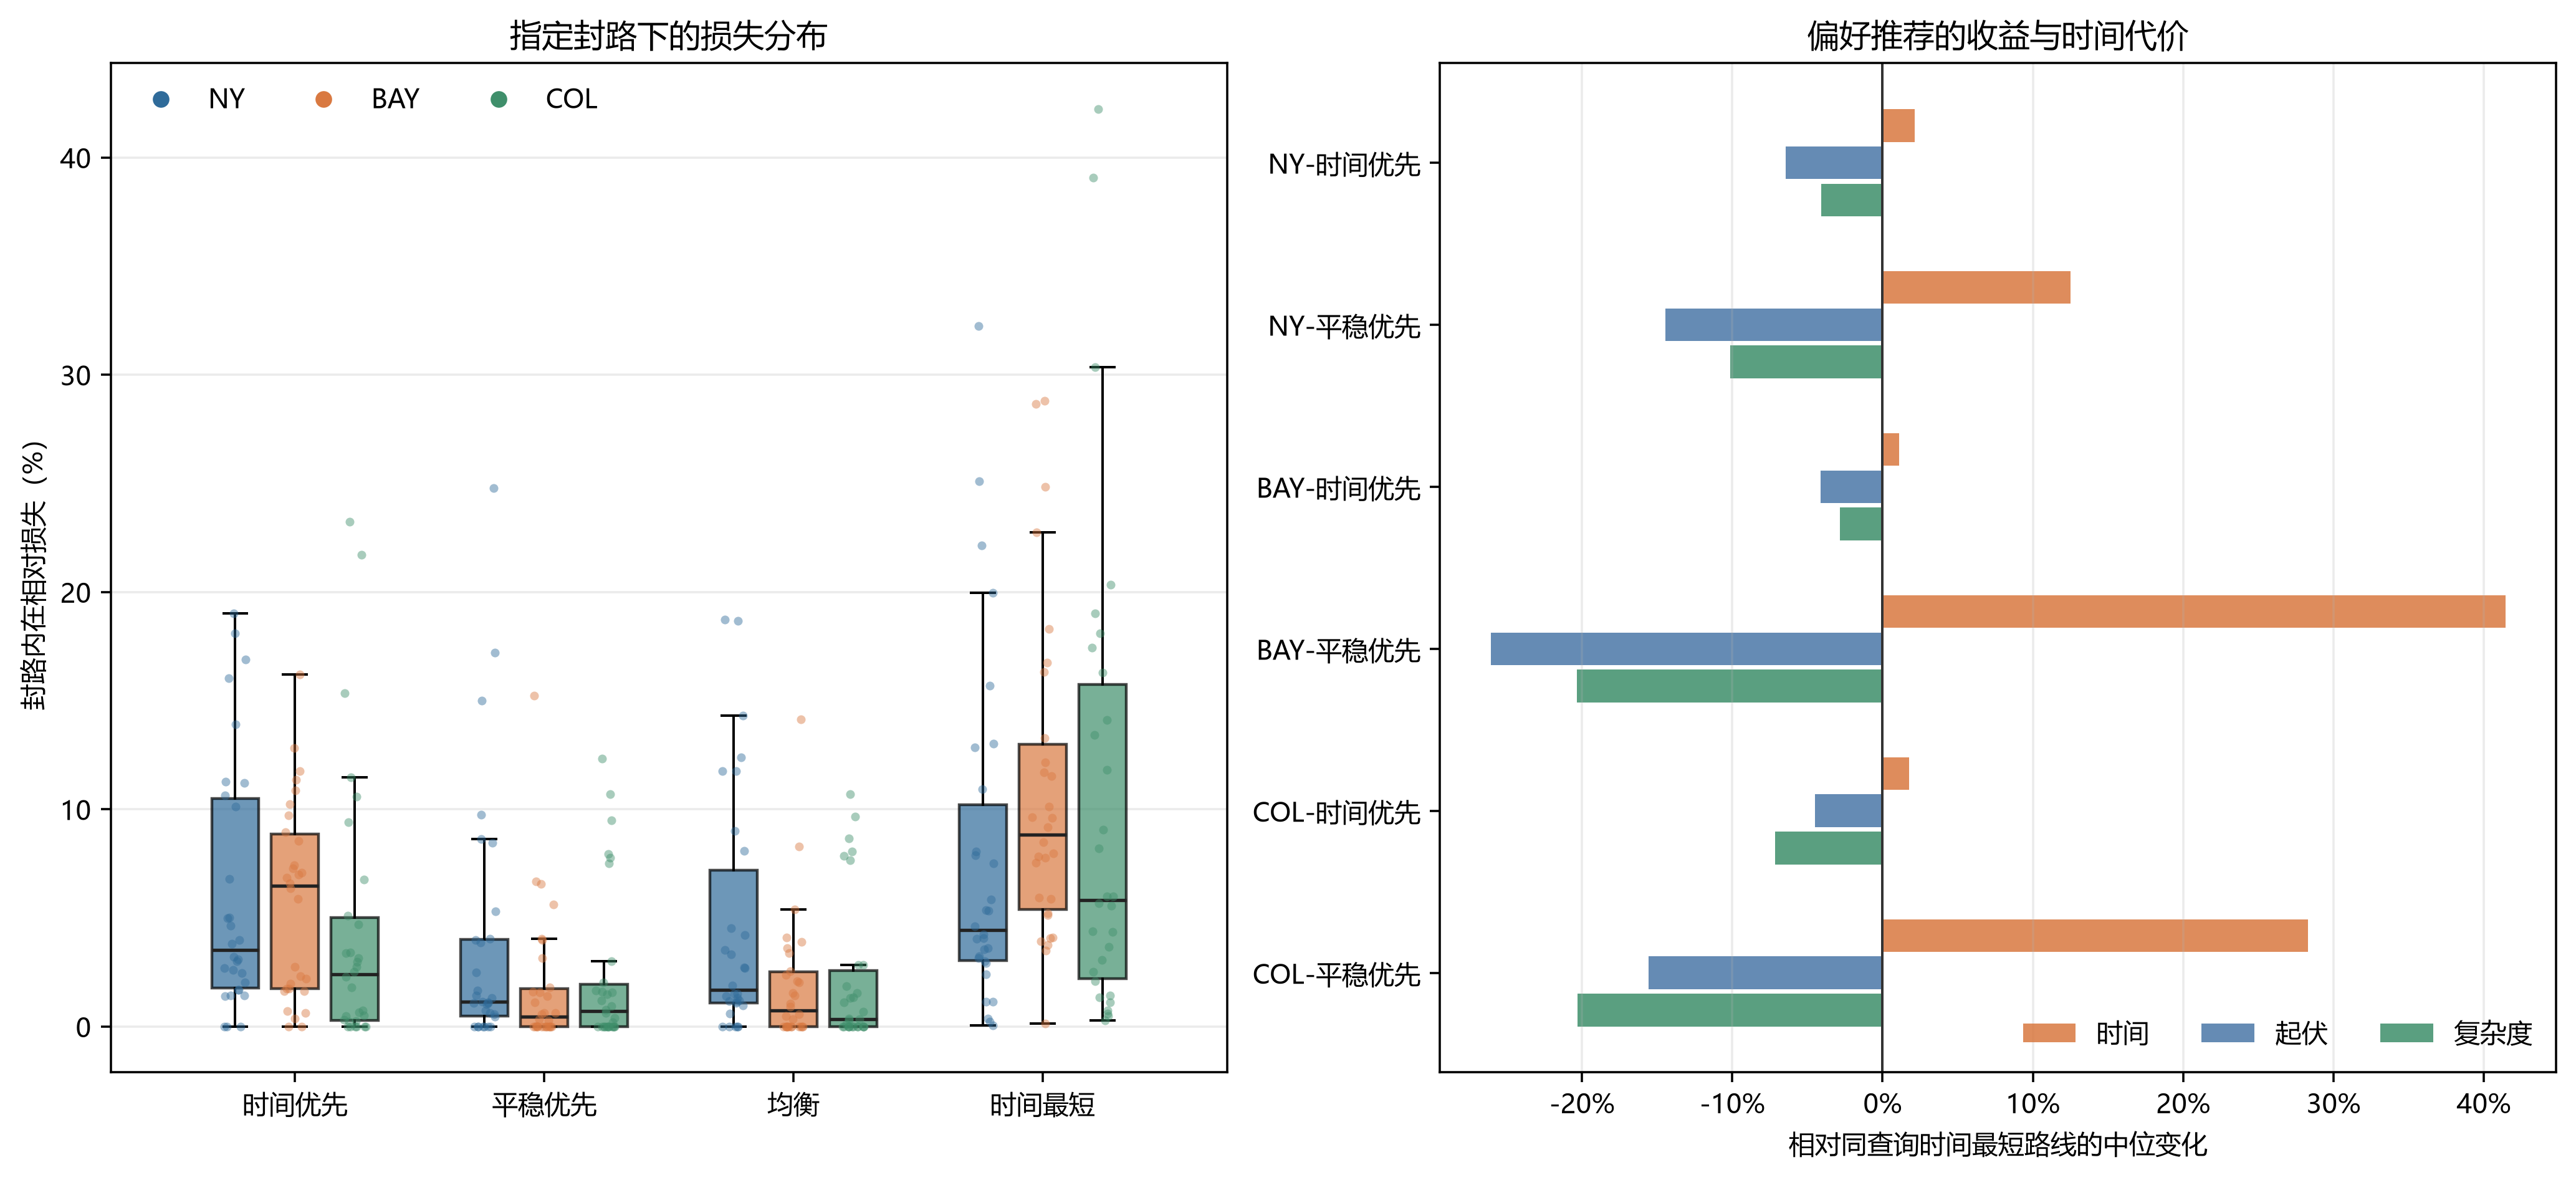
\includegraphics[width=\textwidth]{../figures/q4_closure_and_tradeoff.png}
\caption{封路内在损失分布与偏好推荐的成本权衡}
\label{fig:q4overview}
\end{figure}

原候选加权误差实测最大值为 3.366\%，显著低于五维 20\% 理论界；时间最短方案在全部查询上与原图时间最优值一致。共有 80 个方案实例出现 $W_D^*<W_A$，但全部满足 $W_D^*\ge W_0^*$，验证了“评分下降来自候选近似误差消除，而非封路改善路网”的解释。例如 NY/0001 的均衡方案中，原候选比原图精确最优值高 0.729\%，封路内在损失为 0.600\%；重规划消除的候选误差大于封路增量，故新评分比旧推荐低 0.128\%，但它仍不可能优于原图全局最优值。

\subsection{权重敏感性与计算效率}

分别对“时间权重占比”和“起伏/复杂度合计占比”取 $\theta=0,0.1,\ldots,1$，共完成 $90\times2\times11=1980$ 次选择。表~\ref{tab:q4sensitivity} 显示，时间权重扫描使全部 90 组查询发生过推荐切换；起伏/复杂度扫描使 80 组发生切换。

\begin{table}[H]
\centering
\caption{问题四权重敏感性统计}
\label{tab:q4sensitivity}
\begin{tabular}{lrrrr}
\toprule
& \multicolumn{2}{c}{时间权重扫描} & \multicolumn{2}{c}{起伏/复杂度扫描} \\
\cmidrule(lr){2-3}\cmidrule(lr){4-5}
城市 & 切换查询 & 不同推荐数中位数 & 切换查询 & 不同推荐数中位数 \\
\midrule
NY  & 30/30 & 5 & 28/30 & 3 \\
BAY & 30/30 & 4 & 28/30 & 3 \\
COL & 30/30 & 5 & 24/30 & 3 \\
\bottomrule
\end{tabular}
\end{table}

图~\ref{fig:q4sensitivity} 从每城选取不同推荐数最接近该城中位数的查询。随着时间权重提高，推荐在若干阈值处发生跳变，阈值之间的成本向量保持不变；这与有限候选集上线性评分的分段常值选择结构一致。敏感性实验只覆盖两个一维权重切片，不等同于遍历完整五维权重单纯形。

\begin{figure}[H]
\centering
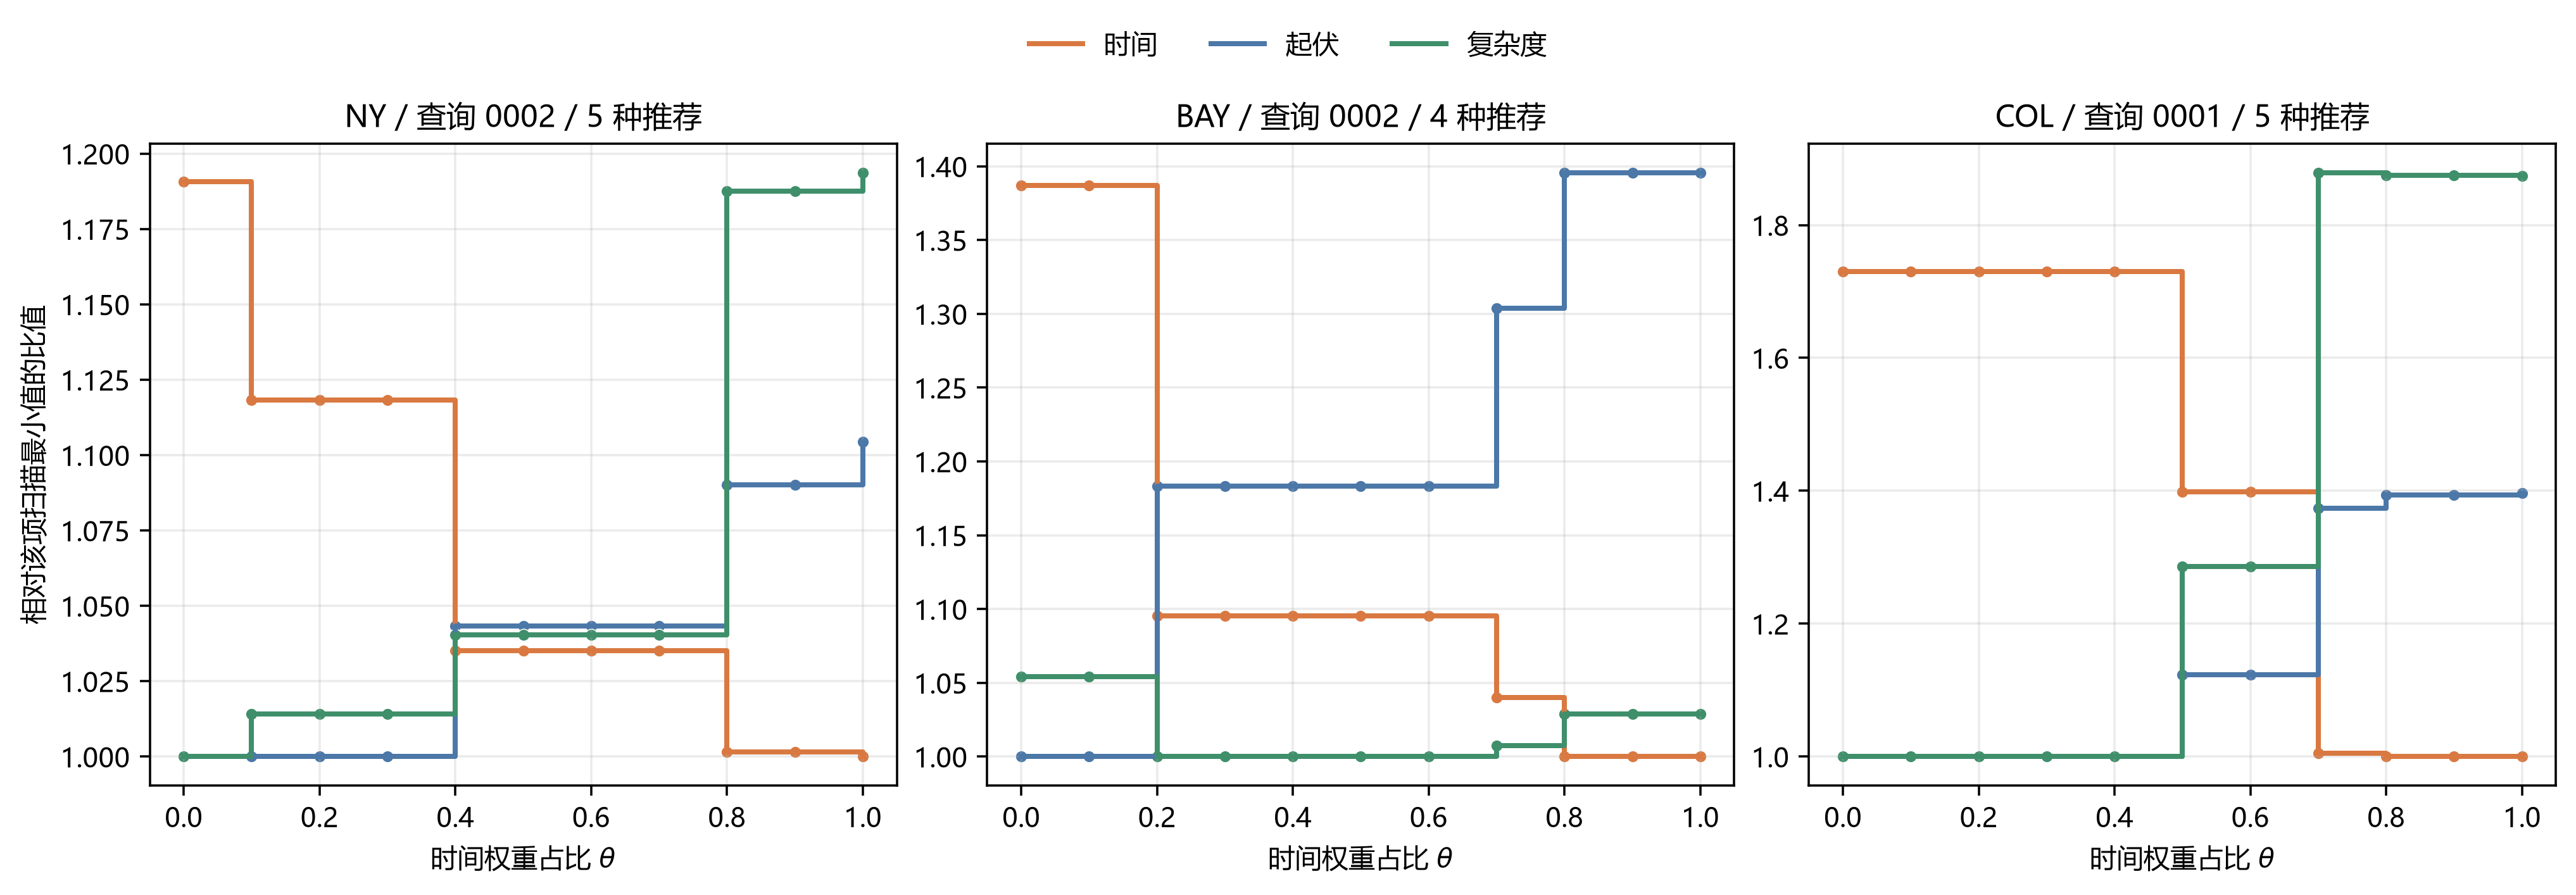
\includegraphics[width=\textwidth]{../figures/q4_sensitivity_examples.png}
\caption{代表查询在时间权重扫描下的推荐切换}
\label{fig:q4sensitivity}
\end{figure}

实验在双路 Xeon Gold 6430、128 逻辑 CPU、约 125 GiB 内存的 Linux 服务器上以 16 个工作进程运行。90 组四方案批次用时 13.942 秒，独立核验另用 42.777 秒。COL 因候选集较大，候选读取、去支配与敏感性选择中位耗时为 0.308 秒；单方案 A* 搜索中位仅为 1.529--6.457 毫秒，但还需约 0.095--0.106 秒的反向预处理，不能把毫秒级 A* 时间当作完整端到端耗时。

\section{模型检验、优缺点与推广}

\subsection{正确性与独立复核}

本文采用“算法不变量证明 + 小图穷举 + 正式结果独立复核”的三级验证：

\begin{enumerate}
  \item 问题二在 2000 个随机有向多重图、六种目标顺序和三种种子设置上，共 36,000 次与简单路径穷举完全一致；
  \item 问题三两个实际使用的内部顺序均通过随机图和多层平行边图穷举，正式 270 组均检查路径、成本、内部非支配和证书状态；
  \item 问题四逐边核验 22,073 条相关路径，并用独立 Python 双向 Dijkstra 复核 720 项最优值；C++ A* 与核验器还分别通过随机/构造小图的穷举对照。
\end{enumerate}

\subsection{模型优点}

\begin{enumerate}
  \item \textbf{保证层次清楚。} 区分精确前沿、乘性覆盖集和固定权重下的精确最优，不把经验质量或可行路径误报为精确结果。
  \item \textbf{适合大规模有向多重图。} 反向下界、降维 skyline 与标签合并显著降低高维搜索开销，并保留实际边编号处理平行边。
  \item \textbf{决策解释一致。} 封路前后固定归一化尺度，区分候选误差、封路内在损失和用户方案变化，避免错误归因。
  \item \textbf{重规划不依赖旧候选存活。} 即使候选全部失效，仍在完整剩余路网上寻找新路线。
\end{enumerate}

\subsection{局限性与改进方向}

\begin{enumerate}
  \item 起伏与节点度只是地形和复杂度代理，尚未包含实时拥堵、道路等级、天气、事故概率和车辆约束；实际部署应接入时变数据。
  \item 问题四权重由情景设定，未通过用户调查或历史选择估计。可采用层次分析、离散选择或偏好学习标定权重，并允许硬约束。
  \item 本文每组偏好单独进行反向预处理。若同终点查询或偏好更新频繁，可缓存势函数，或采用动态最短路与增量搜索方法。
  \item 乘性近似对接近零的目标较敏感；在单位、零值结构不同的应用中，可结合加性误差或混合覆盖指标。
\end{enumerate}

\section{结论}

本文完成了三座大规模真实城市道路网的五维多目标路径规划。单目标结果显示五项指标存在普遍冲突；三目标精确搜索揭示每组可产生上万乃至五万级 Pareto 向量；带真实代表路径的标签合并使全部三、五维查询在 20\% 乘性误差内取得覆盖证书；固定尺度的偏好推荐与完整路网 A* 重规划则在指定封路情景下保持 90 组查询全部可达。

从决策层面看，时间优先方案可以较小时间代价换取一定的起伏与复杂度改善，而平稳优先的时间代价在不同城市差异显著；BAY 对指定封路的最短时间损失中位数最大。时间权重扫描使 90 组查询均发生过推荐切换，表明偏好参数确实改变决策，且路线选择随权重呈阈值式跳变。结果表明，多目标候选、偏好解释和扰动后全图搜索缺一不可：只给单目标路线无法表达权衡，只筛旧候选可能误判不可达，只比较封路前后推荐分数又可能把候选误差误认为路网改善。

\begin{mdframed}
\section*{AI 工具使用说明}
\addcontentsline{toc}{section}{AI 工具使用说明}

本文在研究与写作过程中使用了 OpenAI ChatGPT（GPT-5）及 Codex 辅助工具。AI 主要用于：梳理多目标路径规划的模型结构；辅助检查公式、算法伪代码和文字表述；协助编写、调试数据处理与验证程序；整理实验结果并检查 LaTeX 排版。所有输入数据、算法选择、程序输出、路径合法性、Pareto 性质、近似证书和结论均由作者依据题目材料与独立验证结果复核。AI 工具仅作辅助，论文内容的准确性、完整性与最终学术责任由作者承担。
\end{mdframed}

\renewcommand{\refname}{九、\quad 参考文献}
\addcontentsline{toc}{section}{九、参考文献}
\begin{thebibliography}{99}

\bibitem{dijkstra}
Dijkstra E W. A note on two problems in connexion with graphs[J].
Numerische Mathematik, 1959, 1: 269--271.

\bibitem{astar}
Hart P E, Nilsson N J, Raphael B. A formal basis for the heuristic determination of minimum cost paths[J].
IEEE Transactions on Systems Science and Cybernetics, 1968, 4(2): 100--107.

\bibitem{martins}
Martins E Q V. On a multicriteria shortest path problem[J].
European Journal of Operational Research, 1984, 16(2): 236--245.

\bibitem{namoadr}
Mandow L, P\'erez-de-la-Cruz J L. Multiobjective A* search with consistent heuristics[J].
Journal of the ACM, 2010, 57(5): 1--25.

\bibitem{dimreduce}
Pulido F J, Mandow L, P\'erez-de-la-Cruz J L. Dimensionality reduction in multiobjective shortest path search[J].
Computers \& Operations Research, 2015, 64: 60--70.

\bibitem{apex}
Zhang H, Salzman O, Kumar T K S, et al. A*pex: Efficient approximate multi-objective search on graphs[C].
Proceedings of the International Conference on Automated Planning and Scheduling, 2022, 32: 394--402.

\bibitem{pareto}
Ehrgott M. Multicriteria Optimization[M]. 2nd ed. Berlin: Springer, 2005.

\bibitem{dimacs}
Demetrescu C, Goldberg A V, Johnson D S, eds. The Shortest Path Problem: Ninth DIMACS Implementation Challenge[M].
Providence: American Mathematical Society, 2009.

\end{thebibliography}

\newpage
\section*{附录：核心算法伪代码}
\addcontentsline{toc}{section}{附录：核心算法伪代码}

\subsection*{A. 精确多目标 A*}
\begin{lstlisting}[language={}]
Input: directed graph G, source s, target t, objective count m
Run reverse Dijkstra for every objective to obtain h_j(v)
OPEN <- label (s, g=0), ordered lexicographically by f=g+h
while OPEN is not empty:
    pop the label l with the smallest f
    if a CLOSED label at node(l) dominates l: continue
    insert l into the local skyline
    if node(l)==t: insert its vector into the target skyline
    else for each outgoing edge e:
        l' <- extend(l,e)
        if no target vector dominates f(l'): push l' into OPEN
return target skyline only after OPEN is exhausted
\end{lstlisting}

\subsection*{B. 封路后的偏好重规划}
\begin{lstlisting}[language={}]
Input: original candidates A, closed directed edges F, preference w
Compute L_j and R_j from A; keep them fixed for both networks
Convert normalized preference into exact integer edge weights
Filter all surviving paths in A to obtain a feasible upper bound
Run reverse Dijkstra in the original graph to obtain h_0(v)
Delete every directed edge matching F, including parallel edges
Run A* on the complete disrupted graph using h_0 as heuristic
Stop when the best OPEN lower bound is no better than the incumbent
Reconstruct the path and recompute all five original costs
\end{lstlisting}

\subsection*{C. 结果文件}

四个正式结果文件分别为 \texttt{result1\_研XXX.csv}、\texttt{result2\_研XXX.csv}、\texttt{result3\_研XXX.csv} 和 \texttt{result4\_研XXX.csv}。其中问题一、三、四均输出完整节点序列；问题二输出每组全部不同的三维 Pareto 目标向量。提交前应将文件名中的 \texttt{XXX} 统一替换为实际队号，并保持题目要求的表头与字段顺序不变。

\end{document}
